\chapter{Fase III: Implementación}
\label{cap:Implementacion}

\section{Inicio de sesión y registro de un nuevo usuario}

\begin{figure}[H]
	\centering
	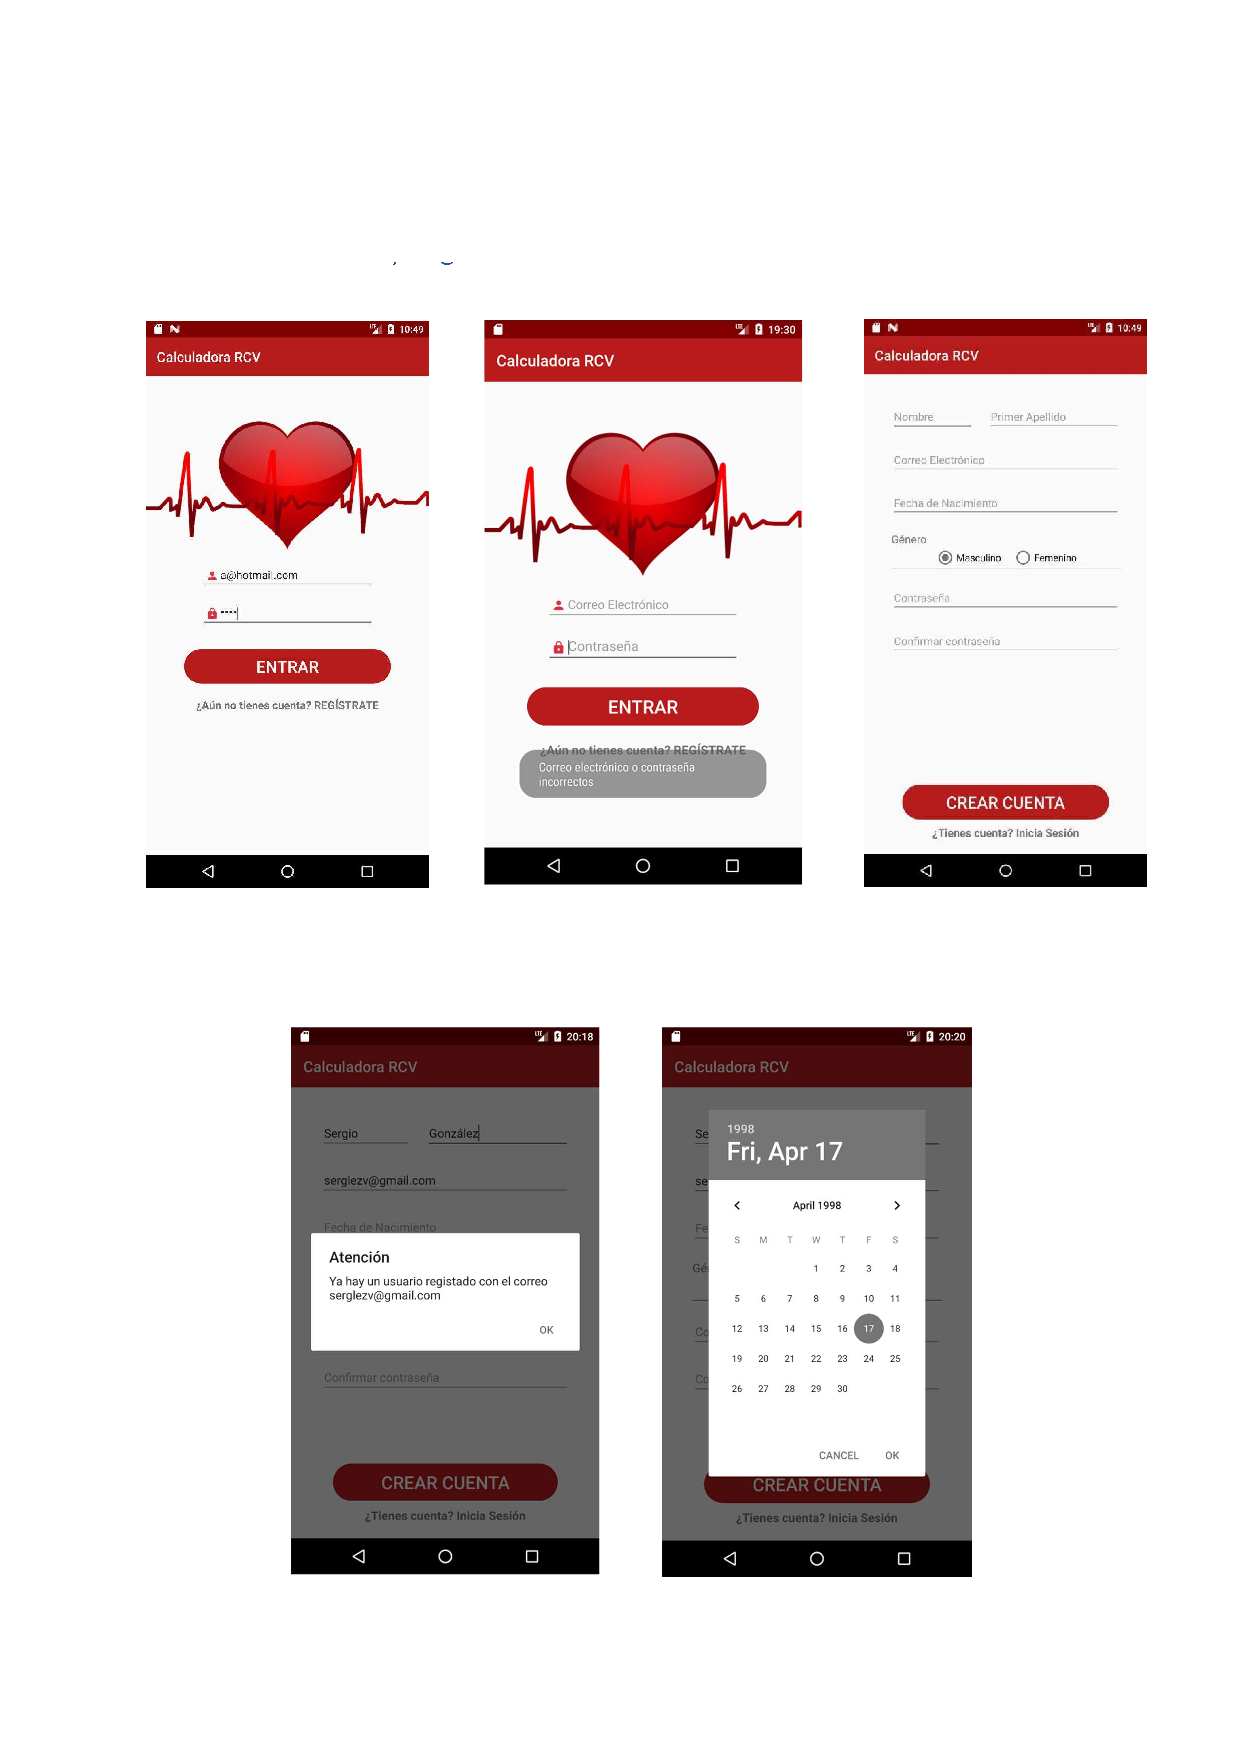
\includegraphics[width=0.9\textwidth]{loginRegistro} 
	\caption[loginRegistro]{Implementación de la ventana para iniciar sesión y registrarse.}
	
	\label{fig:loginRegistro}
\end{figure}



\section{Barra de navegación inferior}

\subsection{Ventana de Estado}
\begin{figure}[H]
	\centering
	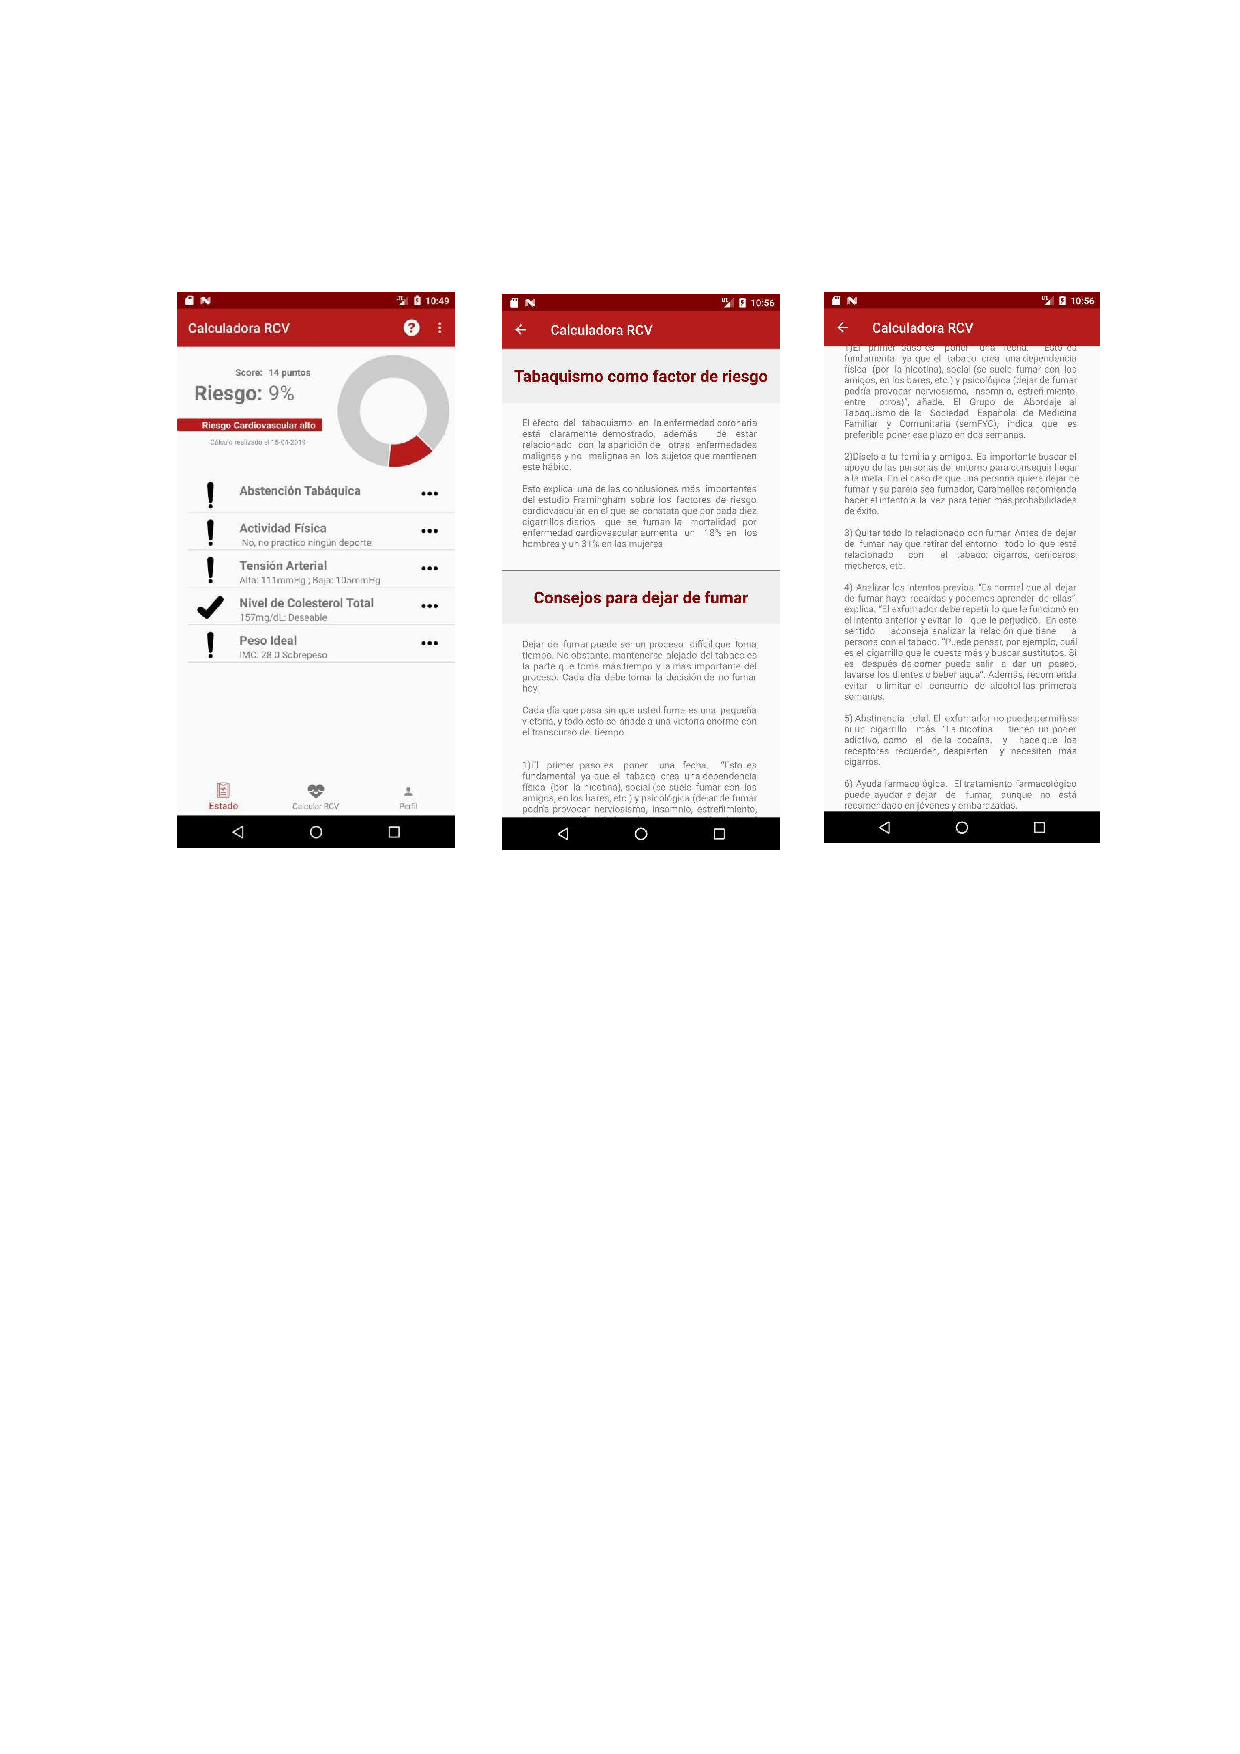
\includegraphics[width=0.9\textwidth]{ventanaEstado} 
	\caption[Implementación Estado]{Implementación de la ventana que informa sobre la última estimación de RCV realizada}
	
	\label{fig:ventanaEstado}
\end{figure}
\subsection{Ventana de nuevo Cálculo}
\begin{figure}[H]
	\centering
	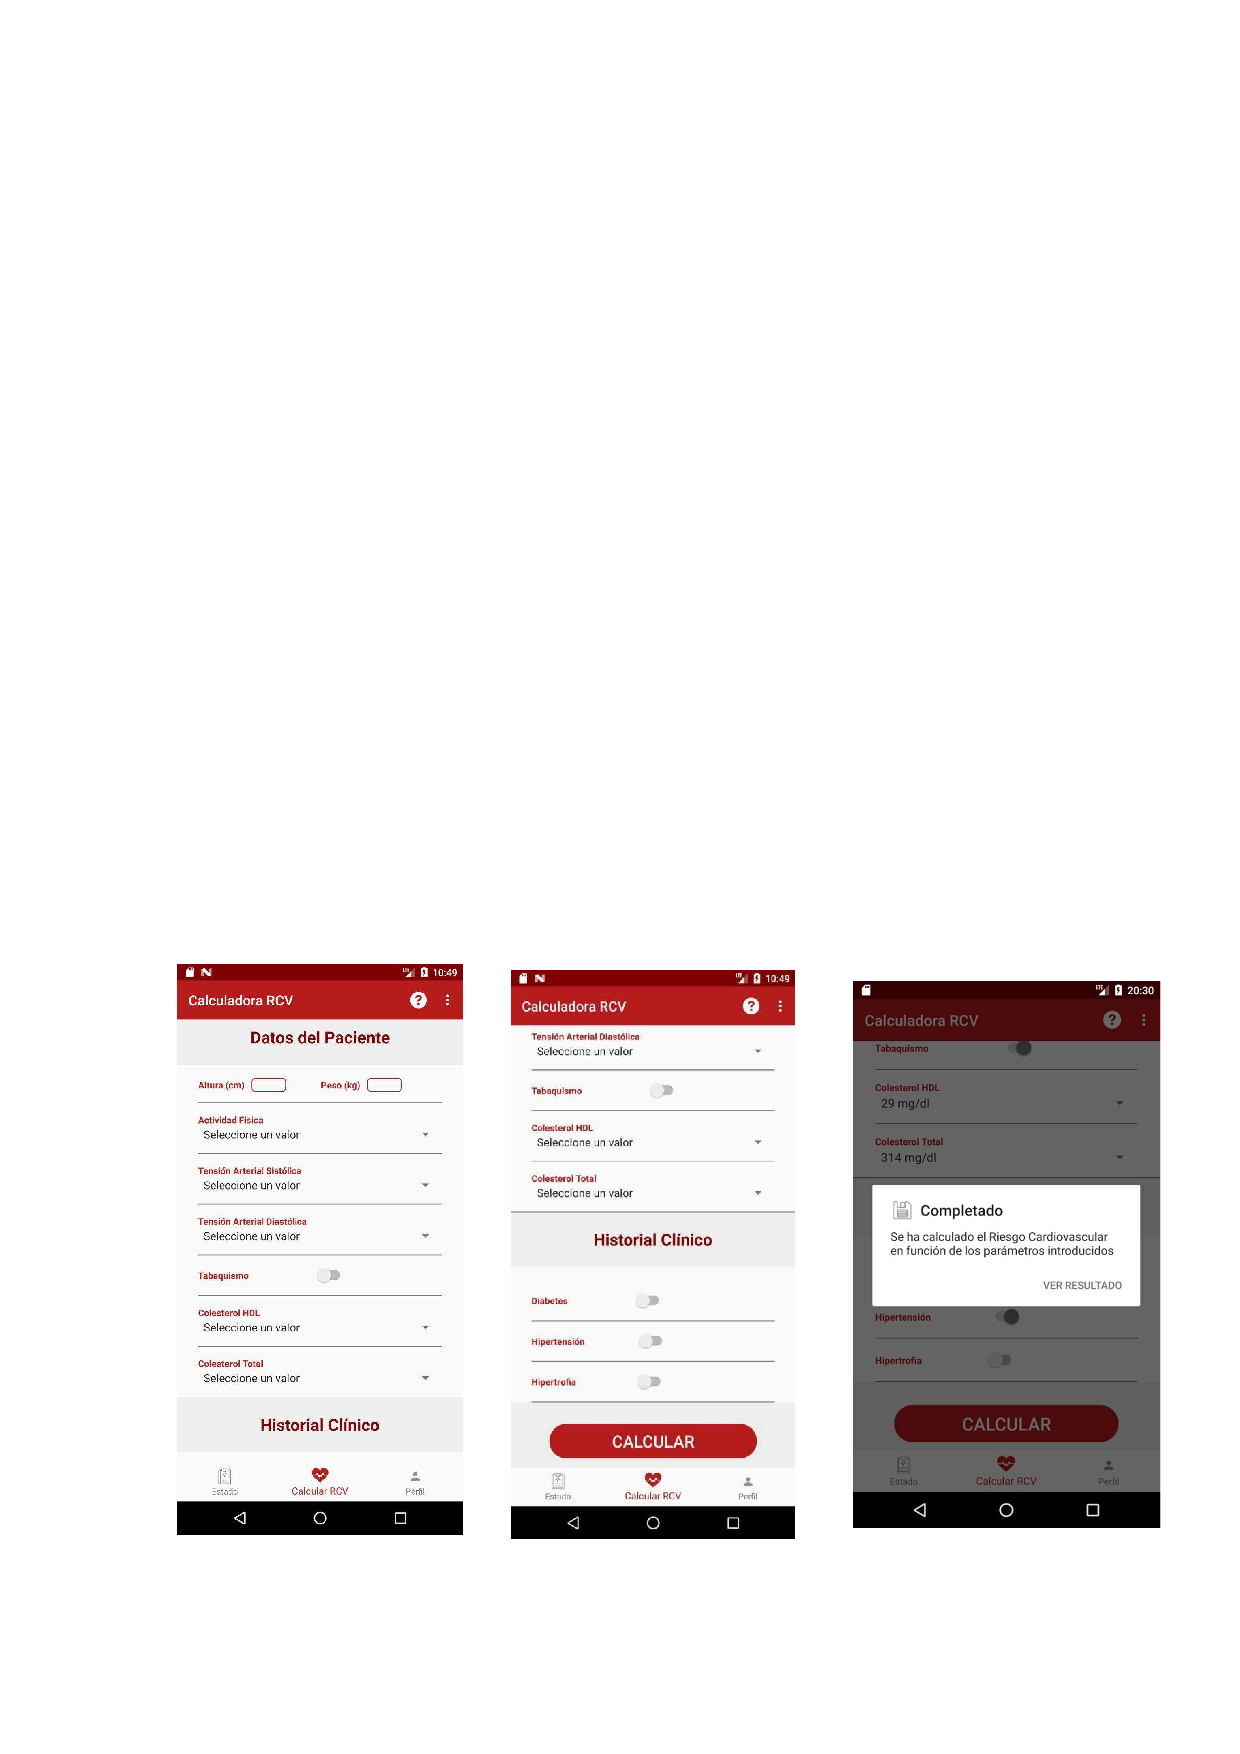
\includegraphics[width=0.9\textwidth]{ventanaCalculo} 
	\caption[Implementación Calculo]{Implementación del formulario para realizar un nuevo cálculo de estimación RCV}

	\label{fig:ventanaCalculo}
\end{figure}
\subsection{Ventana de Perfil}
\begin{figure}[H]
	\centering
	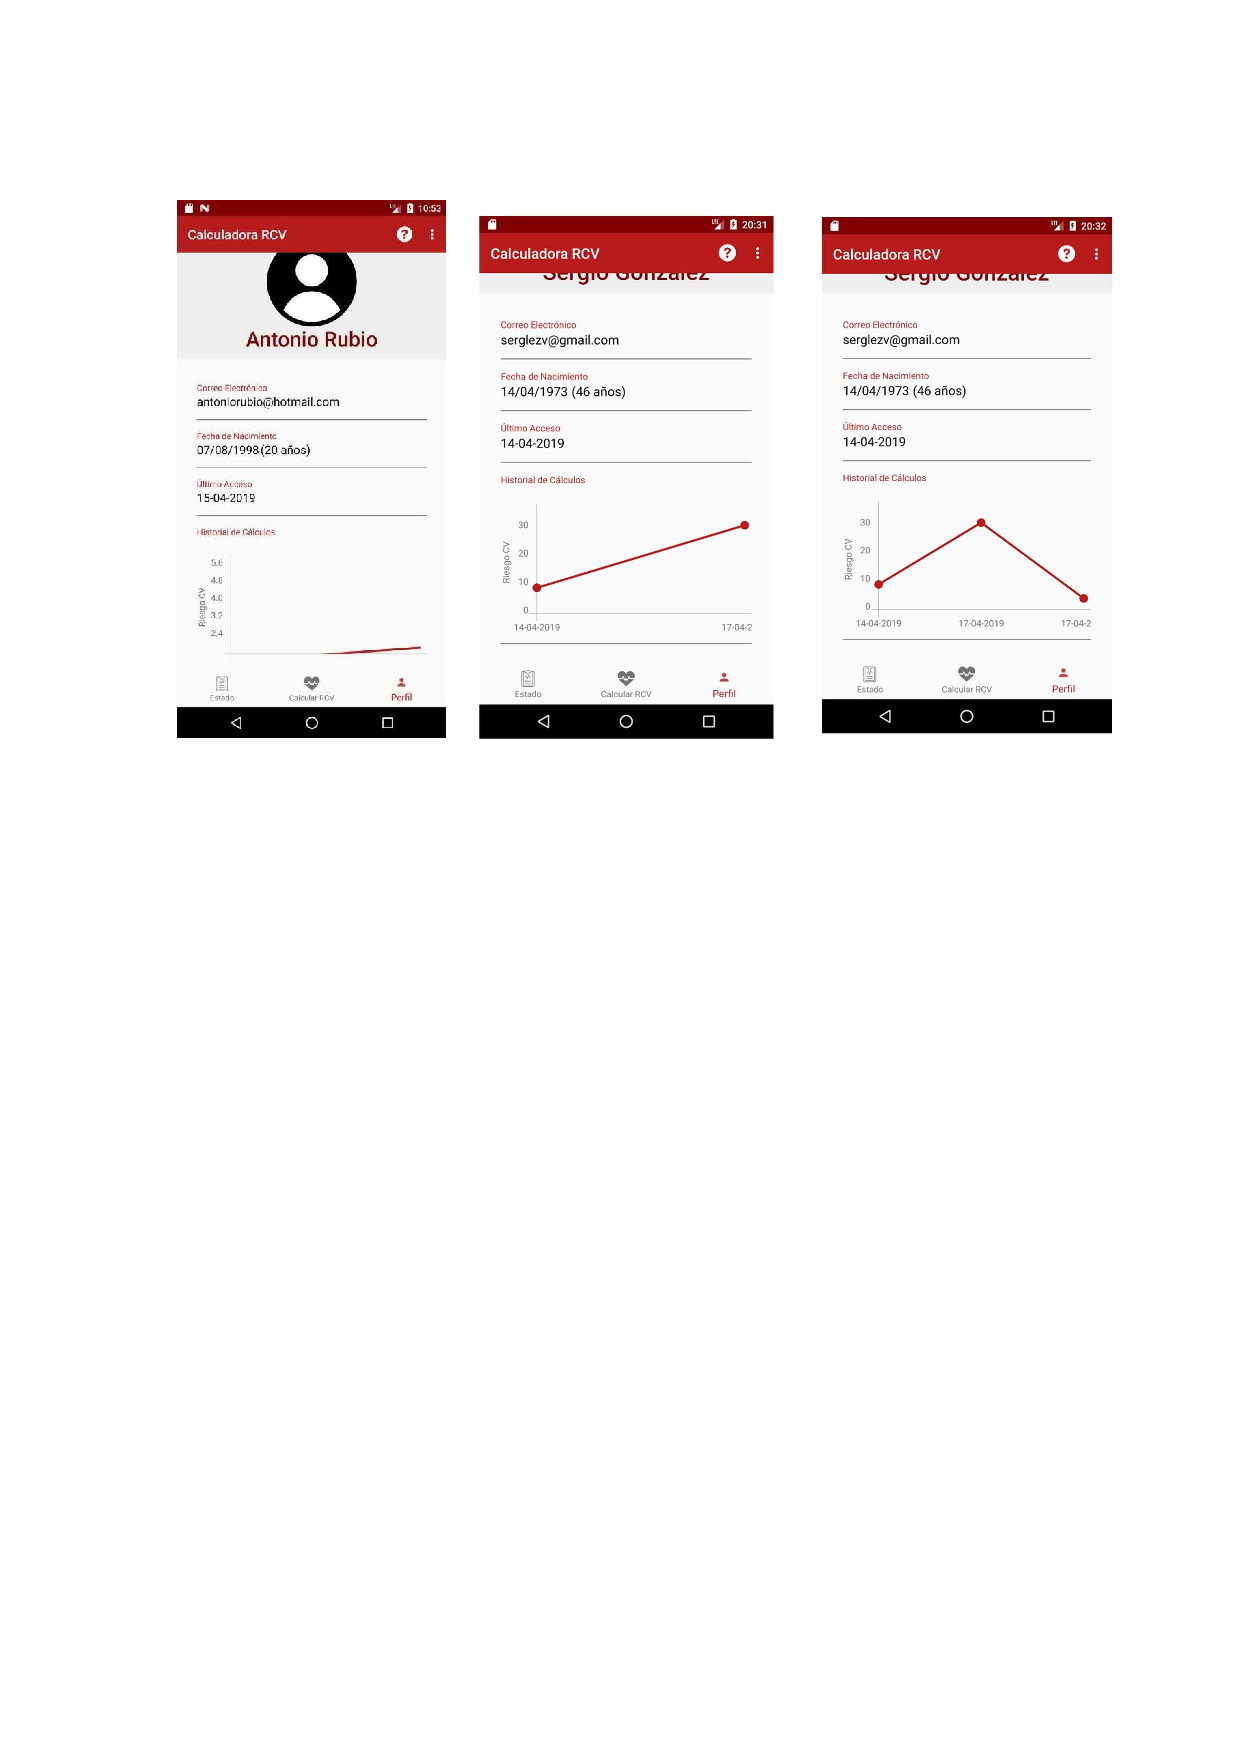
\includegraphics[width=0.9\textwidth]{ventanaPerfil} 
	\caption[Implementación Perfil]{Ventana de perfil en la que se muestra un gráfico que permite monitorizar la evolución del RCV}
	
	\label{fig:ventanaPerfil}
\end{figure}

\section{Action Bar y Acerca De…}
\begin{figure}[H]
	\centering
	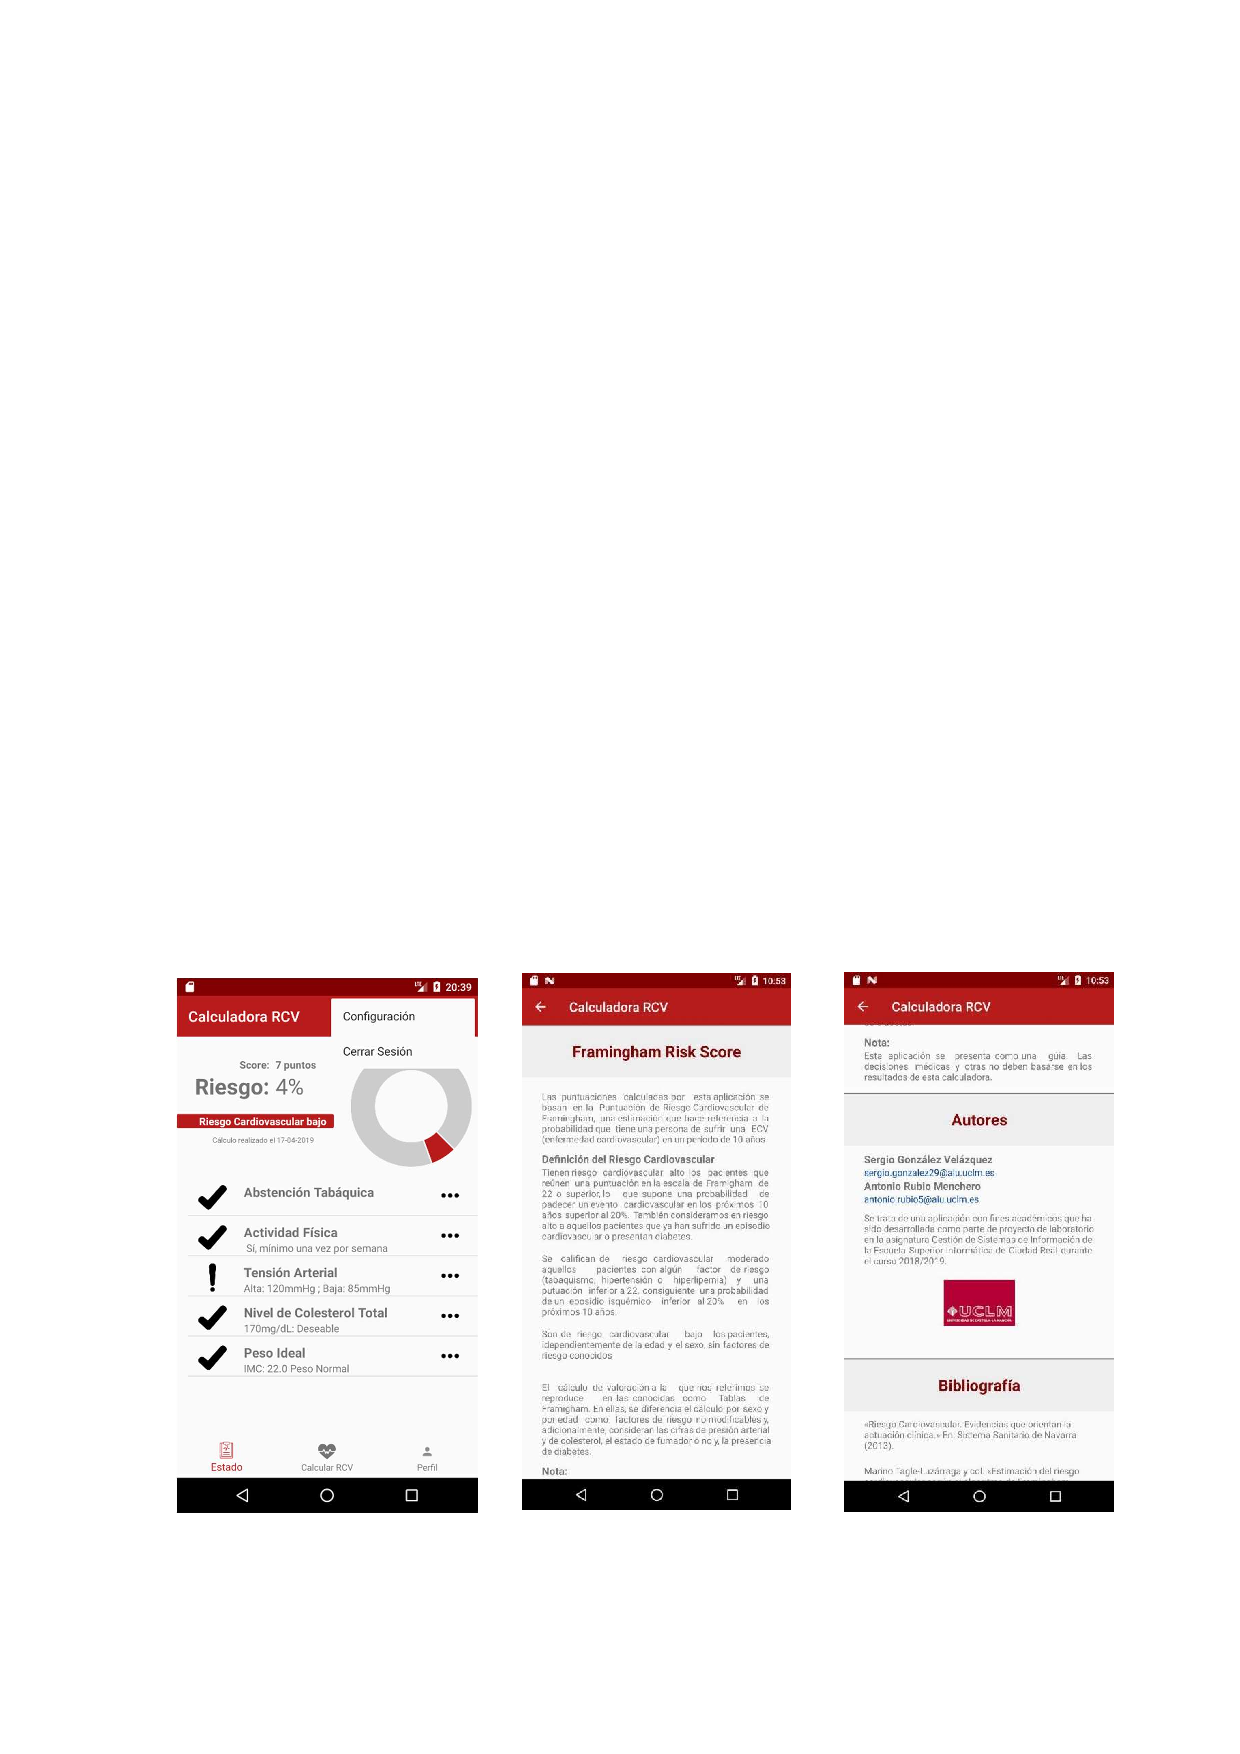
\includegraphics[width=0.9\textwidth]{ventanaActionBar} 
	\caption[Implementación Estado]{Ventana de información y ayuda sobre la aplicación}
	
	\label{fig:ventanaBar}
\end{figure}